\providecommand{\main}{../../../..}
\documentclass[\main/dresen_thesis.tex]{subfiles}
\begin{document}
  \label{sec:looselyPackedNS:layer:vsm}
  \begin{figure}[tb]
    \centering
    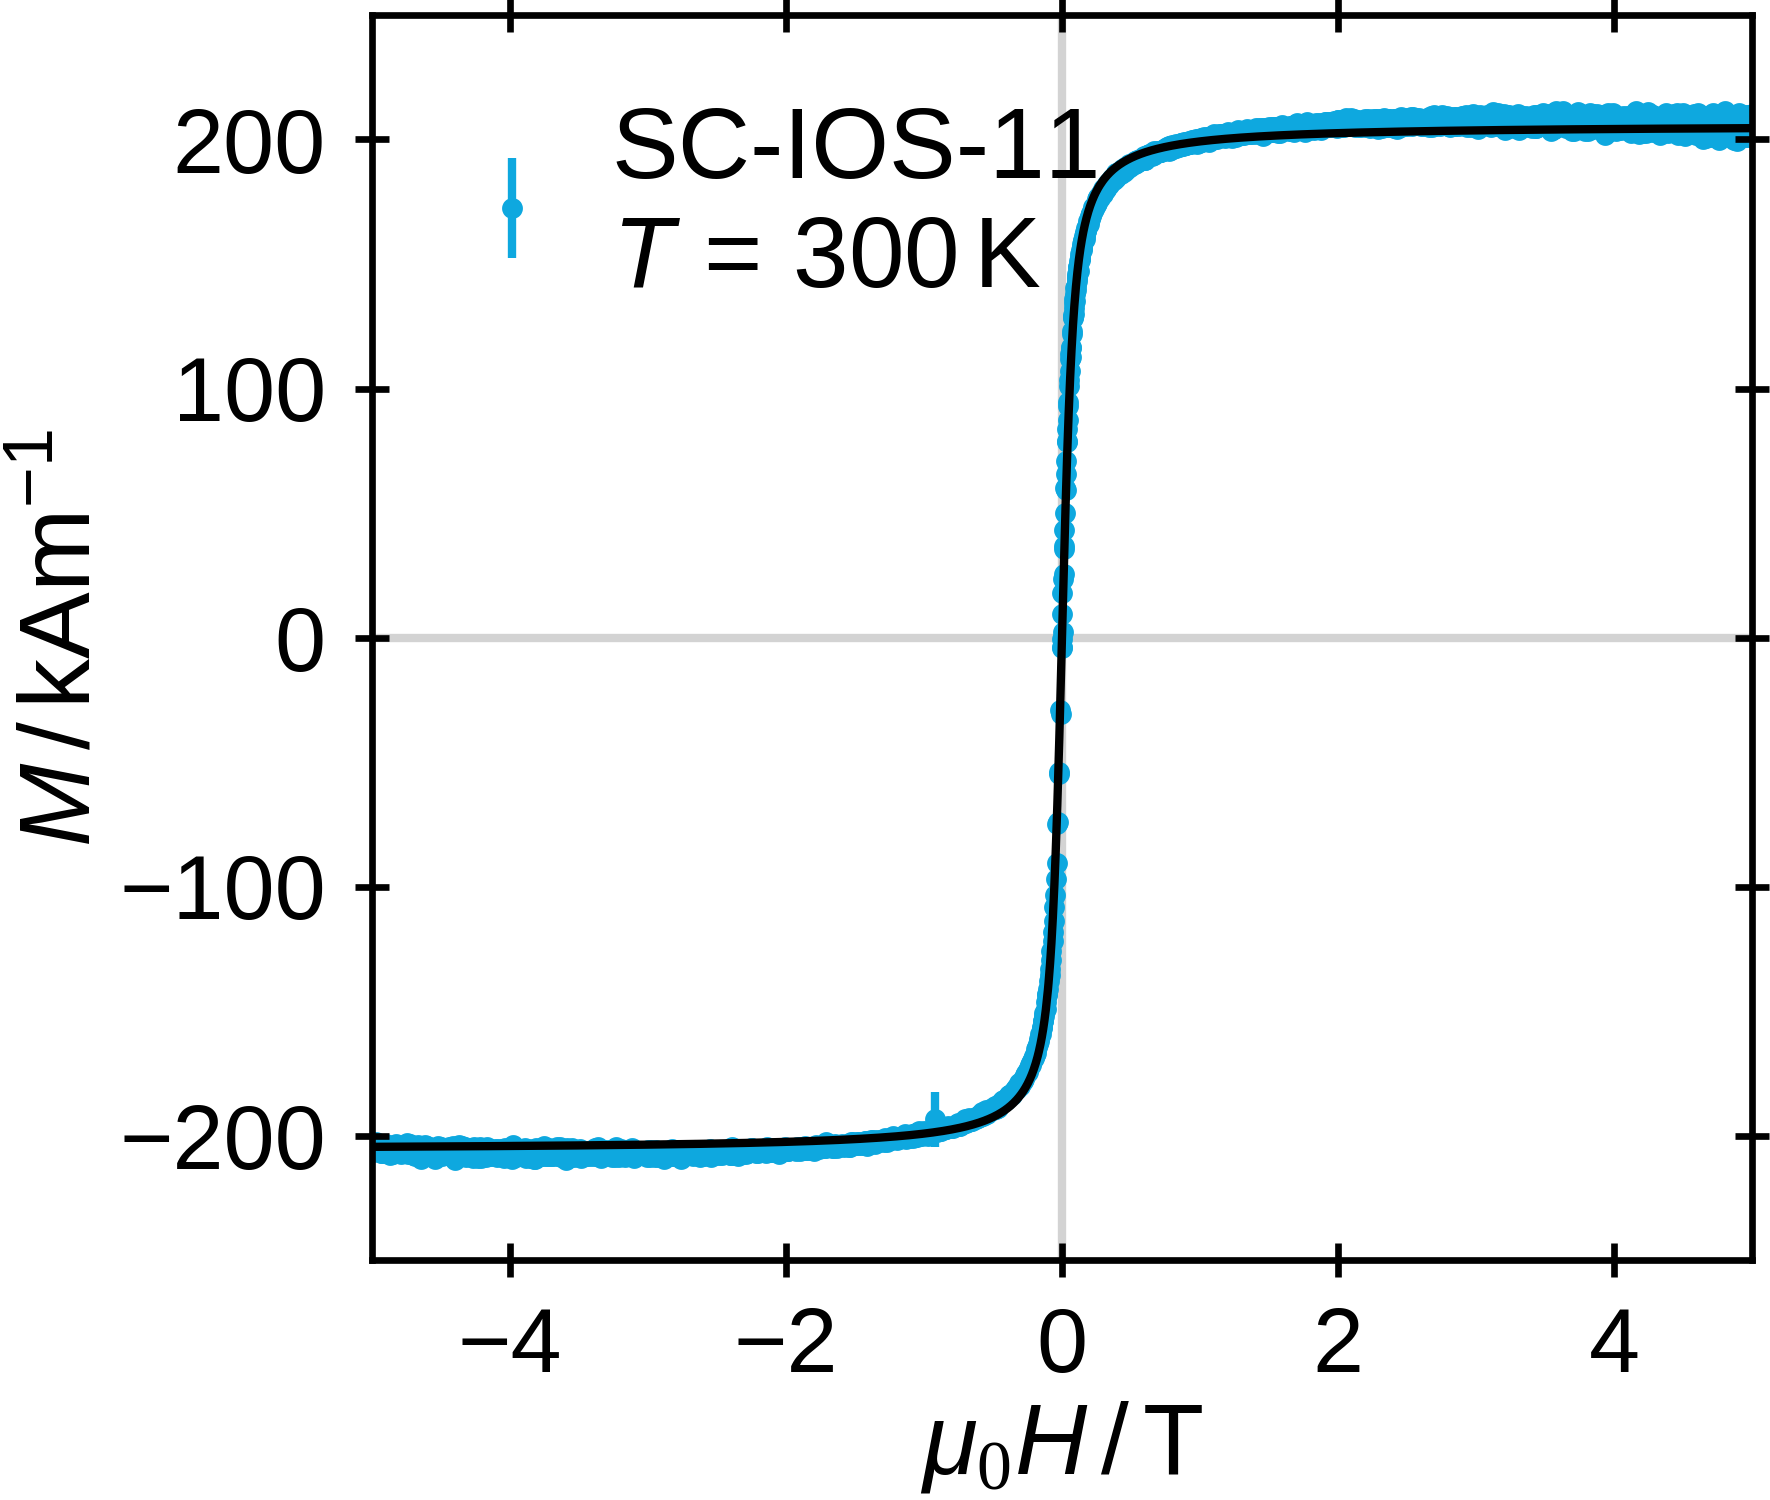
\includegraphics{looselyPackedNP_VSM_SC-IOS-11}
    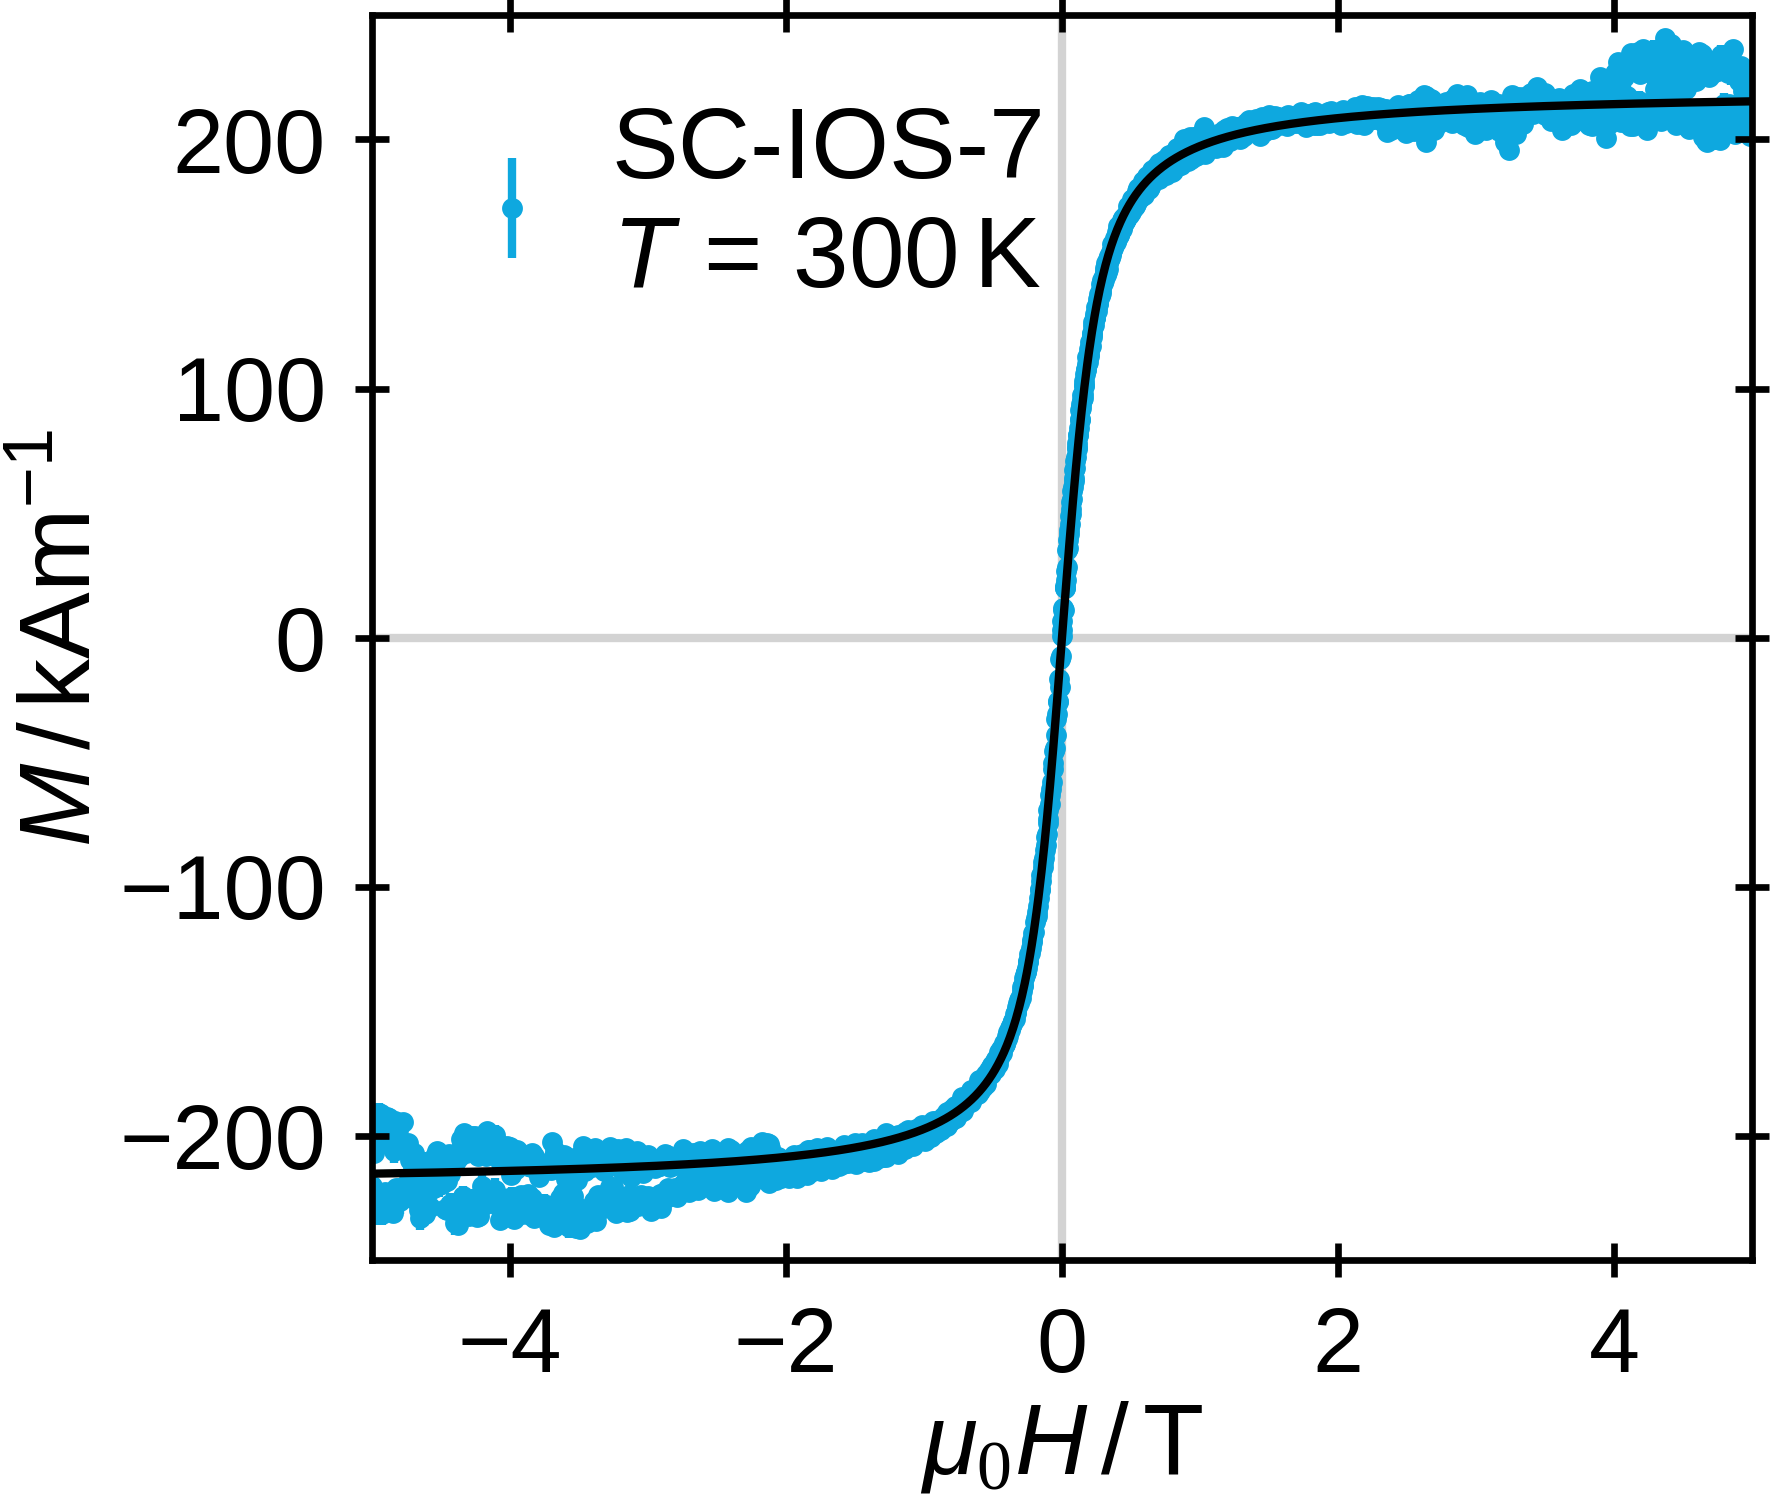
\includegraphics{looselyPackedNP_VSM_SC-IOS-7}
    \caption{\label{fig:looselyPackedNP:layer:vsm}Room temperature vibrating sample magnetometry for SC-IOS-11 (left) and SC-IOS-7 (right). In black a Langevin behaviour is fit and the parameters are given in \reftab{tab:looselyPackedNP:layer:vsm}}
  \end{figure}

  For the magnetic properties of the loosely packed nanospheres, vibrating sample magnetometry provides a method to study the macroscopic magnetization of SC-IOS-11 and SC-IOS-7.
  The field-dependent magnetization of both samples at room temperature is shown in \reffig{fig:looselyPackedNP:layer:vsm}.
  In both cases a superparamagnetic behaviour is observed with no excess susceptibility.
  The magnetization are well described by a Langevin curve with the parameters given in \reftab{tab:looselyPackedNP:layer:vsm}.

  \begin{table}[!htbp]
    \centering
    \caption{\label{tab:looselyPackedNP:layer:vsm}Parameters for the Langevin function shown in \reffig{fig:looselyPackedNP:layer:vsm}, with $\mu$ the magnetic moment and $M_s$ the spontaneous magnetization. Additionally given is the magnetic moment determined for the nanospheres in dispersion $\mu_\mathrm{disp.}$ in \refsec{sec:looselyPackedNS:nanoparticle:vsm}.}
    \begin{tabular}{ c | l | l }
      \rule{0pt}{2ex} \textbf{VSM \@ 300K} & SC-IOS-11 & SC-IOS-7 \\
      \hline
      \rule{0pt}{2ex} $\mu \, / \, \mu_B$           & $13767(51)$   & $4374(16)$\\
      \rule{0pt}{2ex} $M_s \, /  \unit{kAm^{-1}}$   & $205.9(1)$    & $219.8(3)$\\
      \hline
      $\mu_\mathrm{disp.} \, / \, \mu_B$            & $11354(58)$   & $3609(8)$\\
      \hline
    \end{tabular}
  \end{table}
  The determined magnetic moment from the Langevin curve is in both cases approximately $20 \%$ larger than the magnetic moment obtained for the samples measured in dispersion in \refsec{sec:looselyPackedNS:nanoparticle:vsm}.
  % For SC-IOS-11 it is possible that the nanospheres on the silicon substrate have oxidated partially in comparison to the nanospheres in dispersion and therefore a higher magnetization per particle is achieved, and for SC-IOS-7 the obtained value is still in agreement with the result from SANSPOL for IOS-7 (\refsec{sec:looselyPackedNS:nanoparticle:sas}).

  \begin{figure}[tb]
    \centering
    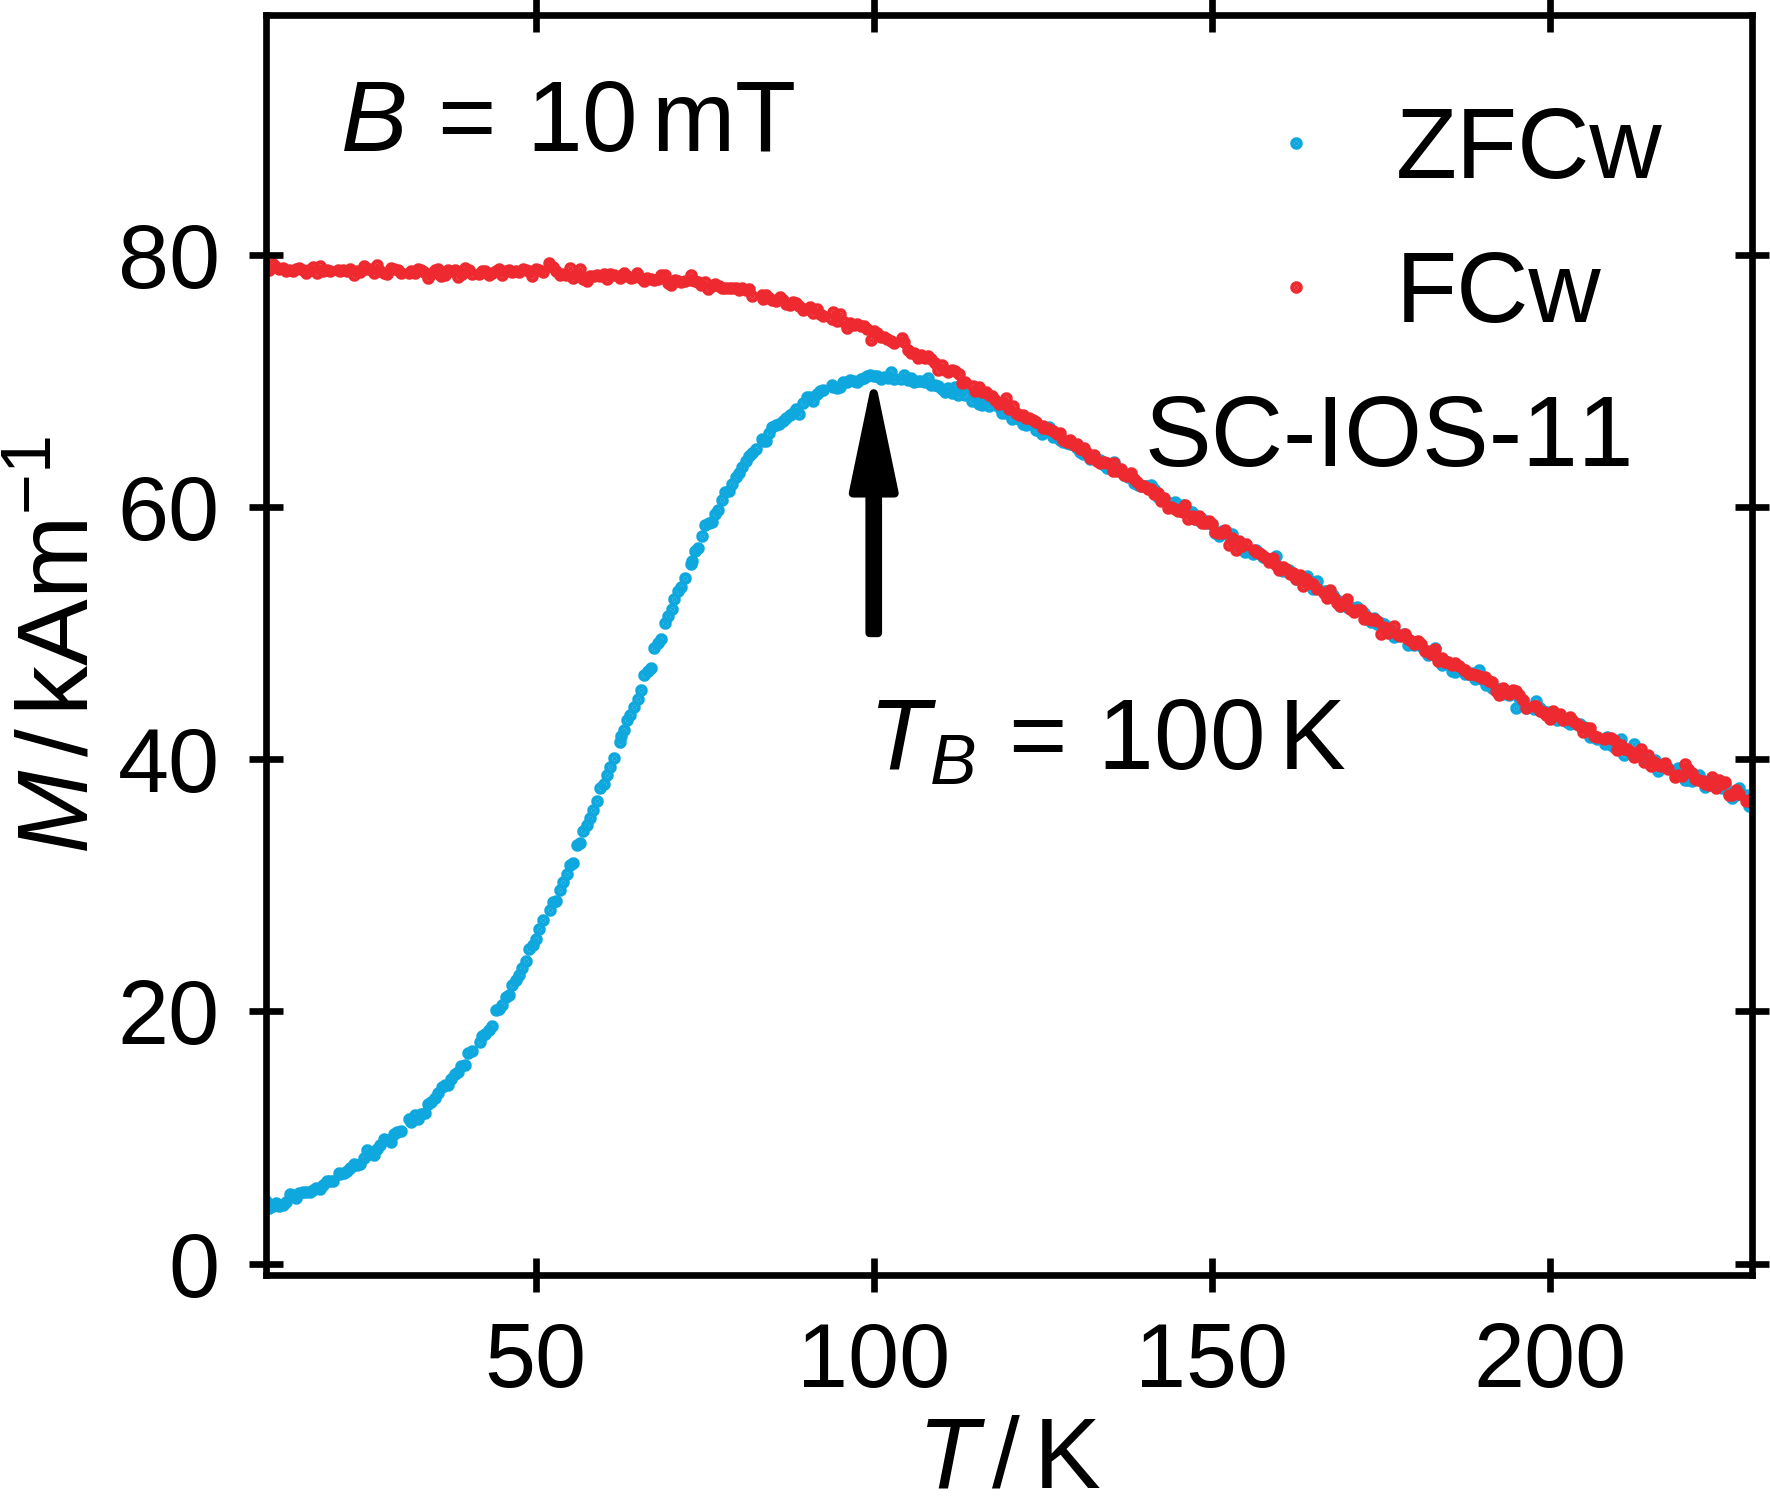
\includegraphics{looselyPackedNP_VSM_ZFC_FC_SC-IOS-11}
    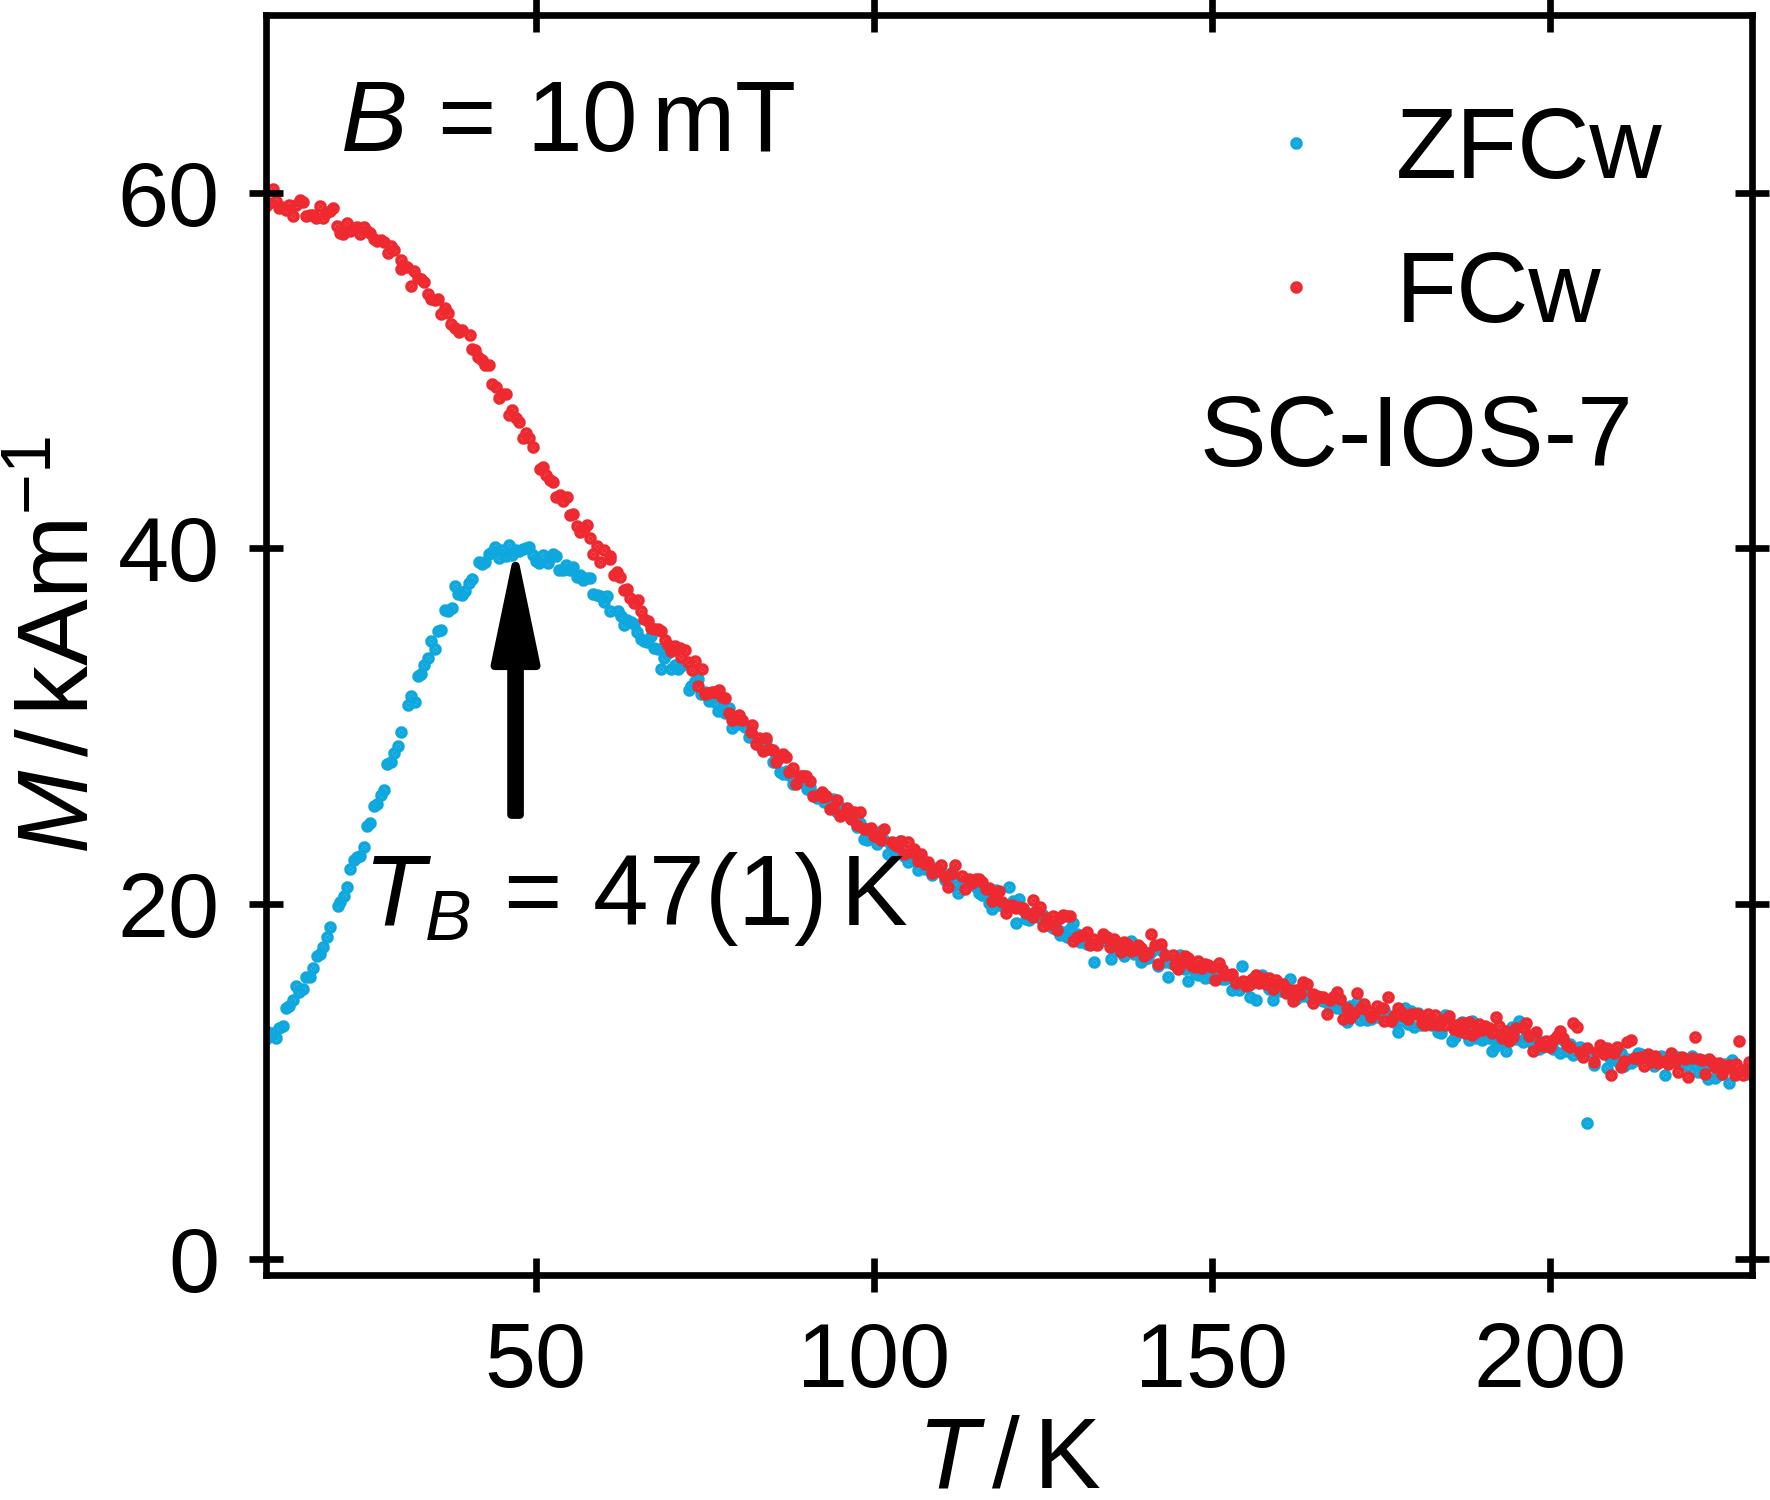
\includegraphics{looselyPackedNP_VSM_ZFC_FC_SC-IOS-7}
    \caption{\label{fig:looselyPackedNP:layer:vsmZFCFC}Temperature dependent magnetization measured at $10 \unit{mT}$ after cooling in zero-field and at a field of $10 \unit{mT}$ for SC-IOS-11 (left) and SC-IOS-7 (right).}
  \end{figure}

  Furthermore, temperature-dependent magnetization measurements of the spin-coated layers are shown in \reffig{fig:looselyPackedNP:layer:vsmZFCFC}.
  The blocking temperature of SC-IOS-11 is determined from the ZFCw measurement to $102(1) \unit{K}$ and for SC-IOS-7 to $47(1) \unit{K}$.
  For SC-IOS-7 the value is well in agreement with the blocking temperature measured for the nanospheres IOS-7 in dispersion (\refsec{sec:looselyPackedNS:nanoparticle:vsm}).
  But for SC-IOS-11 the value is significantly increased in comparison to a blocking temperature of $95.5(5) \unit{K}$ obtained for IOS-11.

  The increased magnetic moment and blocking temperature of SC-IOS-11 indicates a coupling between the spheres, which results in an increased size of the coherent magnetic domains and a higher thermal energy required to turn the sample into the superparamagnetic phase.
  As both macroscopic magnetization measurements of the nanoparticle dispersion and the spin-coated layer have been performed multiple years after the synthesis, it can be assumed that the nanospheres are in both cases in a fully oxidized state as observed in the nanoparticle characterization.

  \begin{figure}[tb]
    \centering
    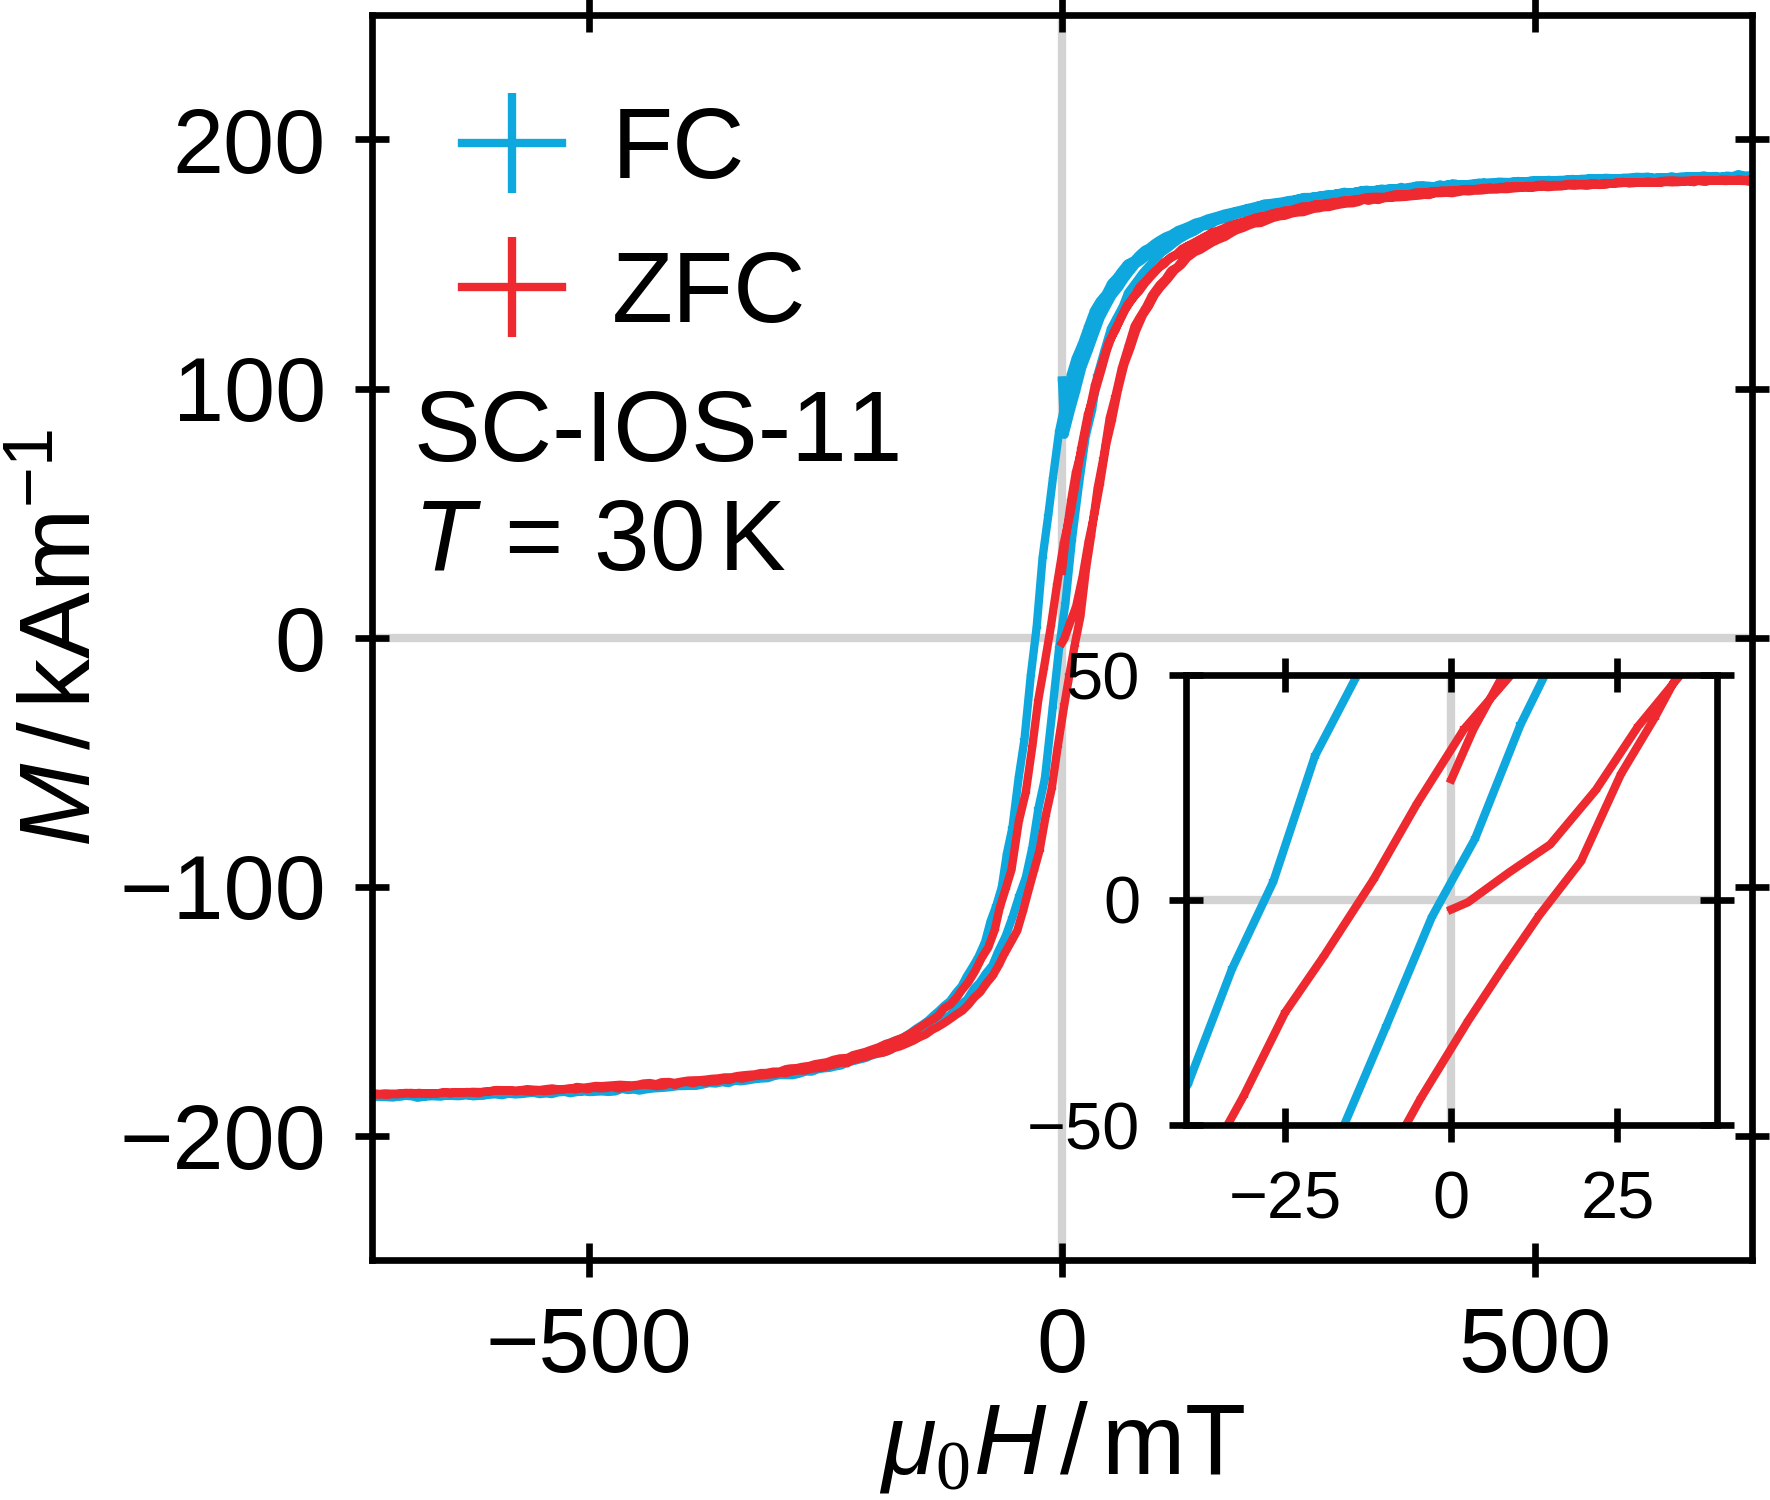
\includegraphics{looselyPackedNP_VSM30K_SC-IOS-11}
    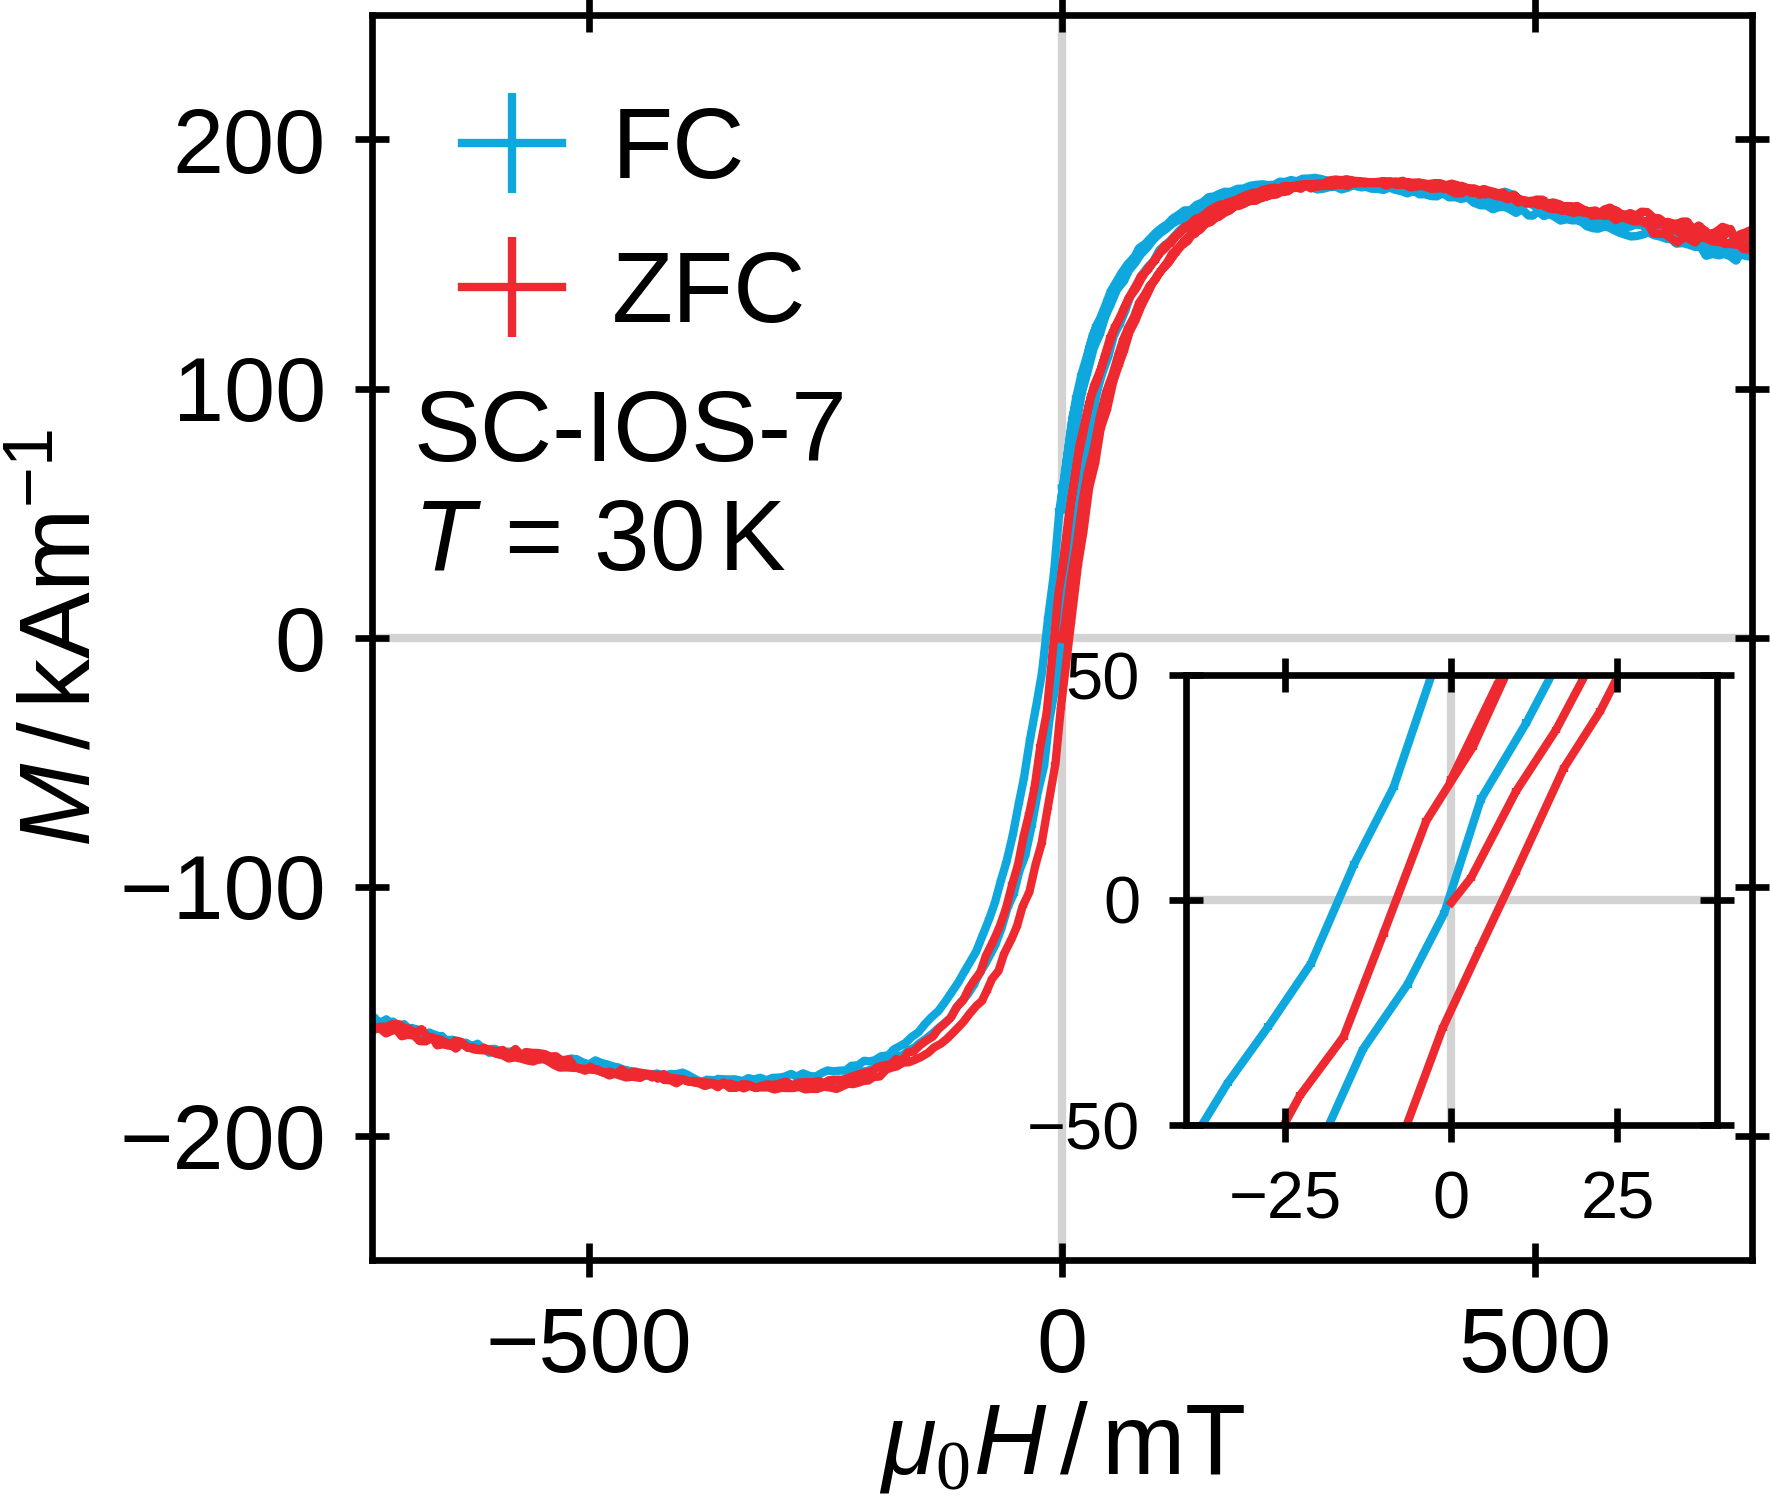
\includegraphics{looselyPackedNP_VSM30K_SC-IOS-7}
    \caption{\label{fig:looselyPackedNP:layer:vsm30K}Temperature dependent magnetization measured at $10 \unit{mT}$ after cooling in zero-field and at a field of $10 \unit{mT}$ for SC-IOS-11 (left) and SC-IOS-7 (right).}
  \end{figure}
  In a next step, polarized neutron reflectometry is therefore used to study the nanostructure magnetization with depth-resolution.
  For the discussion of the reflectivity curves measured at low temperatures, the analogue measurements have been performed on the VSM in \reffig{fig:looselyPackedNP:layer:vsm30K}.
  Both samples have been zero-field cooled and field cooled, before a hysteresis up to a field of $730 \unit{mT}$ is measured at $30 \unit{K}$.
  In both cases a small hysteresis with a coercive field below $20 \unit{mT}$ is visible and the field cooled hysteresis is shifted with respect to the zero-field curve.
  As mentioned in the nanoparticle characterization (\refsec{sec:looselyPackedNS:nanoparticle:vsm}), this shift is also typically observed for the non-interacting magnetite nanoparticles from the oleate synthesis and comes from an exchange-bias effect that originates either from the initial core-shell structure of the nanospheres or after oxidation from the anti-phase boundaries \cite{Wetterskog_2013_Anoma}.




  % At low temperatures the magnetization of IOS-11 and IOS-7 in \reffig{fig:looselyPackedNP:nanoparticle:vsm10} show a hysteretic behaviour, where IOS-11 has a coercive field of $40 \unit{mT}$ and IOS-7 a field of $25 \unit{mT}$.
  % The temperature dependent curves furthermore show the blocking temperature of IOS-11 to be at $100 \unit{K}$ and for IOS-7 at $45 \unit{K}$.
  % The smaller values observed for IOS-7 is connected to the larger population of small-sized nanoparticles, which even at low temperatures are more susceptible to thermal fluctuations.

\end{document}